\documentclass[authoryear,letterpaper,english,12pt]{elsarticle}

\usepackage{comment,color}
\usepackage{array,tabularx}
\usepackage{arydshln} % Dashed array and tabular lines
\usepackage{booktabs,rotating,multirow,framed}
\usepackage{amsthm,
    amsmath,amsfonts,amssymb,xcolor,graphicx,babel,natbib,booktabs,
    chngcntr,comment,array,dcolumn, pdflscape, longtable, pgfplots, rotating, subfigure,
    comment}
\usepackage{colortbl}
\usepackage{hhline}
\usepackage{multicol}
%\usepackage{subcaption}
\usepackage{ulem}    
\usepackage{setspace}

\onehalfspacing

\theoremstyle{plain}
\newtheorem{proposition}{Proposition}
\newtheorem{lemma}{Lemma}
\newtheorem{hypothesis}{Hypothesis}

\numberwithin{lemma}{section}
\numberwithin{proposition}{section}
\numberwithin{equation}{section}
\numberwithin{figure}{section}

\newcommand{\s}{\sigma_2}
\newcommand{\m}{\tilde{\mu}^*_2}
\newcommand{\kap}{z_1(t)}
\newcommand{\D}{\mathrm{d}}

\newcommand{\E}{\mathrm{e}}
\newcommand{\mye}{\ensuremath{\mathsf{E}}}
\newcommand{\R}{\ensuremath{\mathbb{R}}}
\newcommand{\eqdef}{\;\buildrel \text{def}\over =\;}

\newcommand{\alert}[1]{\textcolor{red}{#1}}
\newcommand{\proofpart}[1]{\hfill\break\noindent\textit{#1.}\hspace{3ex}}


\DeclareMathOperator{\var}{var}
\DeclareMathOperator{\cov}{cov}
\DeclareMathOperator{\prob}{prob}
\DeclareMathOperator{\corr}{corr}
\DeclareMathOperator{\stdev}{stdev}

\begin{document}



We study firms with correlated values who have private signals and discretion over when to disclose their signals to the market.  We assume firms wish to maximize their intertemporal average stock prices. Each firm's option to disclose is an American exchange option.  Prior to exercise, each firm is priced by risk-averse investors according to the investors' perception of the firm's value.  The assumption that firms care about average prices means that the price is a ``dividend stream'' received by the firm.  If the firm exercises its exchange option (discloses its signal), then it gives up this dividend stream in exchange for a different dividend stream, namely its price as determined by its private signal.  The value of the asset with which the firm is endowed (its pre-disclosure price) varies stochastically depending on the disclosures of other firms, so each firm's optimal time to exercise depends on the disclosure policies of other firms, each of which in equilibrium also depends on the disclosure policies of others.

This is a particular type of option game.  To our knowledge, this game has not previously been studied.  The static game under risk neutrality dates to Grossman, Milgrom, Dye.  Risk aversion in the static game was introduced by Dye and Hughes but only with a single firm.  Dynamic disclosure is studied by ADK but also with only a single firm and with risk neutrality.  So, our multiple firm model is new both because it includes risk aversion and because it is dynamic.

Equilibrium policies are threshold policies with stochastic thresholds, meaning that at each point in time there is a minimum signal value (threshold), depending on prior disclosures or nondisclosures by other firms, such that it is optimal to disclose if and only if one's signal is above the threshold.  Conditional on a disclosure, there is a nonzero probability that the disclosing firm's signal is exactly equal to the threshold, which we call a ``minimum disclosure.''  It turns out that a key issue in the analysis of the game is whether minimum disclosures make other firms more or less likely to disclose.  This is essentially a question of whether minimum disclosures are good or bad news.  Good news causes prices to rise and makes other firms less likely to disclose; bad news causes prices to fall and make other firms more likely to disclose.\footnote{ADK derive this clustering effect of bad news for exogenous news.}  We show that in the case of two firms, a minimum disclosure is bad news and makes the other firm more likely to disclose.  Based on this result, we characterize the equilibrium fully for the case of two firms.  We conjecture that this result about minimum disclosures applies also for more than two firms.  Conditional on the conjecture, we are able to fully characterize the equilibrium for an arbitrary number of firms.



\section{Model}\label{s:model}




We analyze information disclosure by $n$ firms on a time interval $[0,1]$.  There is a representative investor with constant absolute risk aversion.
Firms learn their date--1 values $\tilde x_i$ at independent uniformly distributed times $\tilde \theta_i \in [0,1]$.  The values are symmetrically and joint normally distributed with the representative investor's date--1 wealth $\tilde w$, which implies that there are constants $\alpha$ and $\beta$ such that, for each $i$,
\begin{equation}
  \tilde x_i =  \alpha + \beta  \tilde w + \tilde \varepsilon_i
\end{equation} 
where the $\tilde \varepsilon_i$ are normally distributed mean-zero variables that are independent of $ \tilde w$.  Assume the $\tilde \varepsilon_i$ are also independent of each other (the single-index model).   Denote the mean and standard deviation of $\tilde w$ by $\mu_w$ and $\sigma_w$, respectively.
Let $\mu= \alpha + \beta \mu_w$ denote the mean of $\tilde x_i$, and let  $\sigma_\varepsilon$ denote the standard deviation of $\tilde \varepsilon_i$.  The variance of $\tilde x_i$ is $\sigma^2 =  \beta^2\sigma_w^2 + \sigma_\varepsilon^2$.  
The correlation of $\tilde x_i$ with $\tilde x_j$ is $\rho = \beta^2\sigma_w^2/\sigma^2$.

Assume the interest rate $r$ is constant.  For convenience, we normalize it to zero.
The stochastic discount factor (SDF) at date 0 for pricing payoffs at date~1 is proportional to the representative investor's marginal utility, which is proportional to  $\E^{-\gamma \tilde w}$.  Because the interest rate is zero, the SDF is 
\begin{equation}
 \tilde m \ = \ \frac{\E^{-\gamma \tilde w}}{\mye[\E^{-\gamma \tilde w}]}\,.
\end{equation}
  We will use risk-neutral pricing.  The risk-neutral expectation of any random variable $\tilde y$ is $\mye^*[\tilde y] = \mye[\tilde m\tilde x]$.
  Assume the information arrival times $\tilde \theta_i$ are independent of $\tilde w$ and hence independent of $\tilde m$.
  
  Lemma~\ref{lemma:riskneutral} states that  the risk-neutral and physical distributions differ only with regard to means, which is a standard result in this CARA/normal setting. The risk premium $\gamma\beta\sigma_w^2$ in Lemma~\ref{lemma:riskneutral} equals risk aversion multiplied by the covariance of the firm value $\tilde x_i$ with the representative investor's wealth~$\tilde w$, as in the CAPM.  The CAPM holds in our model at date~0 but not at subsequent dates, due to the non-normalities induced by investors' inferences.

\begin{lemma}\label{lemma:riskneutral}
Under the risk-neutral probability, the following are true.  The firm values $\tilde x_i$ are joint normally distributed with means $\mu^*  = \mu  - \alpha b\sigma^2$ and with the same standard deviations and correlation as under the physical probability.  Furthermore, they are independent of the information arrival times $\theta_i$, which are independent and uniformly distributed, as under the physical probability.
\end{lemma}  

Assume no information arrives to the market between $0$ and $1$ other than through the disclosures of firms (or the absence of disclosures).  Let $P_t$ denote the price at date $t$ of all firms that have not disclosed (the pool price).  This price evolves deterministically between disclosures and jumps up or down when there is a disclosure.  After a firm discloses, its price is $\tilde x_i$.  

Assume the firm's objective is to choose a disclosure date $\tau \ge \tilde \theta_i$ to maximize
\begin{equation}\label{objective}
 \mye^* \left[\int_0^\tau P_t \,\D t \mid \tilde x_i \right]  + (1-\tau)\tilde x_i \,.
\end{equation}
For any time $t$ prior to $\tilde \theta_i$, the firm has no choice but to remain silent. However, for $t \geq \tilde \theta_i$, it optimally chooses $\tau$ to maximize its price from $t$ onward. The disclosure date $\tau$ is chosen based on all information prior to that date, including the firm's own value and any disclosures made by other firms. Our choice of the objective function \eqref{objective} is motivated by the assumption that the firm or its managers benefit from having a higher share price over the course of time until date~1. For simplicity, we assume the benefit is additive in time and that the benefit is valued according to the market's SDF, producing the objective \eqref{objective}.

We need to work with the conditional distributions that arise as firms disclose their values.  It is convenient to define these inductively.  Put subscripts $n$ on the unconditional parameters $\mu$, $\mu^*$, $\sigma$, and $\rho$.  This indicates that there are $n$ firms that have not yet disclosed.  Order the firms in the reverse order of disclosure, so firm $n$ is the firm that discloses first, etc.  For any $1< k \le n$, define
\begin{subequations}\label{parameter_recursion}
\begin{align}
\mu_{k-1}(\tilde x_k, \ldots \tilde x_n) \ & = \ \rho_{k} \tilde x_{k} + (1-\rho_{k})\mu_{k}(\tilde x_{k+1},\ldots \tilde x_{N})\\
\mu^*_{k-1}(\tilde x_k, \ldots \tilde x_Nn) \ & = \ \rho_{k} \tilde x_k + (1-\rho_{k})\mu^*_{k}(\tilde x_{k+1}, \ldots \tilde x_{n})\\
\sigma_{k-1} \ & = \ \sigma_{k}\sqrt{1-\rho_{k}^2}\\
\rho_{k-1} \ & = \ \frac{\rho_{k}}{1+\rho_{k}}\,. \label{rhon}
\end{align}
\end{subequations}

\begin{lemma}
Conditional on $\tilde x_{k+1}, \ldots, \tilde x_n$, the random variables $\tilde x_{1}, \ldots, \tilde x_k$ are joint normal under the physical probability with means $\mu_k(\tilde x_{k+1}, \ldots \tilde x_n)$, standard deviations $\sigma_k$ and correlation $\rho_k$.  The distribution is the same under the risk-neutral probability except that the means are $\mu^*_{k}(\tilde x_{k+1}, \ldots \tilde x_n)$.
\end{lemma}

\section{Equilibrium}

We consider `threshold strategies,' meaning that at each date $t$, there is a random variable $B_t$, depending on information at $t$, such that each firm $i$ that has received its signal and has not disclosed at $t$ will disclose at $t$ if and only if $\tilde x_i \ge B_t$.  This is equivalent to assuming that if a firm with signal $x$ chooses to disclose at $t$, then all firms with signals $y>x$ will also  disclose.  There is greater urgency for firms with high values to disclose, because they lose more by trading at prices below their values, so the assumption that higher types disclose first is very natural.

We assume that the threshold or boundary $B_t$ is a continuous decreasing function of time between disclosure dates.  The assumption that it is decreasing is motivated by the fact that the price will be decreasing between disclosure dates, because as time passes it becomes more likely that firms have received their signals, and nondisclosure then indicates that the signals are low.  The boundary can jump up or down when a firm discloses, depending on the content of the disclosure.

%%%%%%%%%%%%%%%%%%%%%%%%%%%%%%%%%%%%%%%%%%%%%%%%%%%%%%%%%%
%
\subsection{Equilibrium Price}
%
%%%%%%%%%%%%%%%%%%%%%%%%%%%%%%%%%%%%%%%%%%%%%%%%%%%%%%%%%%

We can express the price in terms of the history of the boundary.  For each date $t$ and each $s<t$, define
$$C_{st} \ = \  \min_{s\le u \le t} B_u\,.$$
This is the `forward looking' minimum of the boundary at date $s$, looking forward through~$t$.  It matters for pricing because the market knows at $t$ that some firm(s) may have received its signal before $t$ -- say, at $s<t$ -- and has not yet disclosed because its signal was below the threshold at all dates between $s$ and $t$.  This means that its signal is below $C_{st}$.  Because the market does not know the date $s$ at which the firm received its signal (or even if it has received a signal at all) it has to integrate over $s$.  As a result of these calculations, the equilibrium price is as follows.  Let $\phi$ and $\Phi$ denote the standard normal density and distribution function respectively.  The integrals in \eqref{price} below are actually finite sums, because $C_{st}$ is a step function in $s$.  The number, timing, and sizes of steps depend on the history of disclosures.  

\begin{proposition}\label{prop:price}
At any date $t$, let $k$ denote the number of firms that have not yet disclosed and denote the disclosures of the other firms by $x_{k+1},\ldots, x_n$.  
The price of the firms that have not disclosed is
\begin{equation}\label{price}
P_t \ = \  \left[\mu^*_k - \sigma_k\frac{\int_0^t \phi\left(\frac{\mu^*_k-C_{st}}{\sigma_k}\right)\,\D s}{1 - \int_0^t \Phi\left(\frac{\mu^*_k-C_{st}}{\sigma_k}\right)\,\D s}\right]\,,
\end{equation}
where we use $\mu^*_k$ as shorthand for $\mu^*_k(x_{k+1},\ldots, x_n)$.  
\end{proposition} 

\subsection{The Disclosure Option}\label{ss:option}

When multiple firms have correlated values and some have not yet disclosed, it may be optimal for a firm to continue to exercise plausible deniability even after the pool price drops below its value. This is due to the possibility that another firm may become informed, disclose a high value, and cause the pool price to jump upwards, which prolongs the value of plausible deniability.  In other words, like typical American options, the disclosure option must be sufficiently far in the money before it is optimal to exercise it.\footnote{\citet*{adk} describe this same real option effect relative to the exogenous announcement that they study.  The difference in our model is that all announcements are endogenous.  Each firm takes into account the option values created by others, and, in turn, each firm's optimal reaction to the option value affects the options values of all other correlated firms.}

We analyze this disclosure option like any other American option. The optimal disclosure threshold is determined by a differential equation in the inaction region, in conjunction with value matching and smooth pasting conditions at the boundary of the region.     At each date~$t$ after a firm learns its value $\tilde x_i$, define the value function
\begin{equation}\label{Jt}
J_t \ = \  \sup_\tau \; \mye^*_t \left[\int_t^\tau P_u \,\D u \mid \tilde x_i \right] + (1-\tau)\tilde x_i\\,.
\end{equation}
The supremum in \eqref{Jt} is taken over disclosure times that can depend on all prior information, and the value \eqref{Jt} depends on all prior disclosures and on the firm's value $\tilde x_i$.  

We can rewrite \eqref{Jt} as
\begin{equation}\label{Jt2}
\mye^*_t\left[ \int_t^1 P_u \,\D u \mid \tilde x_i \right] + \sup_\tau \; \mye^*\left[\int_\tau^1(\tilde x_i - P_u)\,\D u \mid \tilde x_i\right]\,.
\end{equation}
The second term in \eqref{Jt2} is the value of an American exchange option in which the firm exchanges the reward process $P_u$ for $\tilde x_i$.  The formulation \eqref{Jt2} is natural from an option-pricing point of view, but another formulation is also interesting.  We can  write \eqref{Jt} as:
\begin{equation}\label{Jt3}
(1-t)\tilde x_i + \sup_\tau \; \mye^*\left[\int_t^\tau (P_u-\tilde x_i )\,\D u\mid \tilde x_i\right]\,.
\end{equation}
The first term in \eqref{Jt3} is the value the firm would achieve if disclosure were mandatory, and the second term is the value of plausible deniability.

Bellman's Principle of Optimality implies that the stochastic process
\begin{equation}\label{martingale}
\int_0^t P_u\,\D u + J_t
\end{equation}
is a martingale under the risk-neutral probability.
Taking the differential of \eqref{martingale}, we see that the martingale property of \eqref{martingale} can be stated as
\begin{equation}\label{hjb}
P\,\D t + \mye^*[\D J] \ = \ 0\,.
\end{equation}
The value $J_t$ is determined by equation \eqref{hjb} in conjunction with value matching and smooth pasting. 
The value matching condition is that, at the optimal disclosure time $t=\tau$,
\begin{equation}\label{vm}
J_t \ = \ (1-\tau)\tilde x_i\,.
\end{equation} 
The smooth pasting condition at the boundary is that $J$ paste together smoothly (in~$x$) with the value on the right-hand side of \eqref{vm}. 


We show in \ref{app_foc} that equation \eqref{hjb}, value matching, and smooth pasting are equivalent to a simple marginal condition for the exercise boundary.  Consider a firm with value $\tilde x_i$ such that $\tilde x_i > P_t$.  In other words, the firm would trade at a higher price if it disclosed.  The cost of delaying disclosure for an instant $\D t$ is $(\tilde x_i -P_t)\,\D t$.  The benefit of delaying disclosure is that another firm may disclose a high value during the instant $\D t$, lifting the pool price and producing a positive jump $\Delta J_t$ in $J_t$.\footnote{For a firm at the optimal exercise boundary, downward jumps in $J_t$ are not possible, because a  downward jump in the boundary does not affect the optimal policy of a firm that is already at the boundary -- the firm should still disclose, so the value of $J$ is still the right-hand side of \eqref{vm} after such a jump.  On the other hand, an upward jump in the boundary means that it is optimal to continue to exercise plausible deniability a while longer, so the value of $J$ becomes larger than the right-hand side of \eqref{vm}, that is, there is a positive jump $\Delta J_t$.}    The marginal condition is that the costs and benefits of delaying disclosure must be equal for a firm at the boundary.  Therefore, the equilibrium exercise boundary at date $t$ is the number $B_t$ such that the probability another firm discloses at $t$ times the expected value of $\Delta J_t$ conditional on a disclosure equals the cost $(B_t-P_t)\,\D t$ of delaying disclosure.  

\subsection{The Last Firm}

We can in principle find the equilibrium inductively, starting with the last firm to disclose and working backwards.  The last firm will disclose as soon as the price falls below its value, because there is no value to keeping its disclosure option alive.  So, the value function for the last firm, conditional on a value $\tilde x_1$ is
\begin{equation}\label{value:last}
    J_t = \int_t^1 (P_u \vee \tilde x_1)\,\D u\,,
\end{equation}
where $P$ denotes the equilibrium price process, which depends on the disclosures of the other $n-1$ firms.  Using \eqref{price} and the fact that the price and boundary are the same for the last firm, we obtain the following characterization of the price $P_u$.  

\begin{proposition}\label{prop:last}
Let $t$ denote the date at which the penultimate firm discloses.  Let $c_1< \cdots < c_j$ denote the distinct values of $C_{st}$ for $s<t$ and let $\Delta_1,\ldots, \Delta_j$ denote the lengths of the intervals on which $C_{st}=c_i$ for $i=1,\ldots,j$.
Set $\mu^*_1 = \mu^*_1(\tilde x_2,\ldots,\tilde x_N)$.  For each $u\ge t$ and for $k=1,\ldots, j+1$, consider the fixed-point problem:
\begin{equation}
z_k \ = \ \frac{\sum_{i=1}^{k-1} \phi\left(\frac{\mu^*_1-c_i}{\sigma_{1}}\right)\Delta_i + \phi(z_k)\left[u- \sum_{i=1}^{k-1}\Delta_i\right]}
{1 - \sum_{i=1}^{k-1} \Phi\left(\frac{\mu^*_{1}-c_i}{\sigma_{1}}\right)\Delta_i - \Phi(z_k)\left[u- \sum_{i=1}^{k-1}\Delta_i\right]}
\end{equation} 
There is a unique positive solution $z_k(u)$.  It is increasing in $u$ for each $k$.  Furthermore, 
\begin{equation}
P_u  \ = \ \mu_1^* - \sigma_1 \max_{k=1,\ldots,j+1}z_k(u)\,.
\end{equation}
\end{proposition}

\subsection{Induction}

Given the value function when there are $k-1$ firms remaining, we can compute the jump in value when there are $k$ firms remaining and one of the $k$ firms discloses.  Thus, we may be able to solve the marginal condition to compute the boundary and hence the value function when there are $k$ firms remaining.  If so, then we should be able to proceed this way until we have backed up to the start when there are $n$ firms remaining.  We implement this for $n=2$ in the next section to display some properties of the equilibrium.  

\section{Solution with Two Firms}

Suppose $n=2$.  Let $t$ denote the date at which the first firm discloses, and let $c$ denote the boundary just before its disclosure.  We denote the post-disclosure price by $P^*$ to distinguish it from the price prior to either firm disclosing.  The post-disclosure price at $u>t$ is given in Proposition~\ref{prop:last} as
\begin{equation}\label{price:last}
    P^*_u = \mu_1^* - \sigma_1 \max(z_1(u), z_2(u))
\end{equation}
where the $z_k$ are the fixed points in
\begin{align}
z_1 \ &= \ \frac{u\phi(z_1)}{1 - u\Phi(z_1)}\\
z_2 \ &= \ \frac{ t\phi\left(\frac{\mu^*_1-c}{\sigma_{1}}\right)+ (u-t)\phi(z_2)}
{1 - t\Phi\left(\frac{\mu^*_{1}-c}{\sigma_{1}}\right) - (u-t)\Phi(z_2)}
\end{align}

Now suppose that at some date $t$ neither firm has yet disclosed.  From Proposition~\ref{prop:price}, the price of each firm is
\begin{equation}
    P_t = \mu^*_2 - \sigma_2 \frac{t \phi\left(\frac{\mu^*_2 - B_t}{\sigma_2}\right)}
    {1 - t \Phi\left(\frac{\mu^*_2 - B_t}{\sigma_2}\right)}\,.
\end{equation}

Our next result simplifies the task of finding the equilibrium boundary $B_t$ prior to either firm disclosing.

\begin{proposition}\label{prop:keylemma}
Suppose the first firm discloses $\tilde x_1 = B_t$, where $B_t$ is the equilibrium boundary prior to either firm disclosing.  Then, the post-disclosure price \eqref{price:last} for the remaining firm is no higher than $B_t$.
\end{proposition}

Now, we can calculate the boundary $B_t$ prior to either firm disclosing by solving the marginal condition described in Section~\ref{ss:option}. 
Suppose one firm knows its value $\tilde x_2$, which is at the boundary $B_t$.  The cost of delaying disclosure is $(B_t-P_t)\,\D t$.  By value matching, the firm's value is $(1-t)B_t$.  There is a jump in the value at $t$ only if the other firm learns its value at $t$ and the value is sufficiently high to produce a post-disclosure price \eqref{price:last} that exceeds $B_t$.  In this case the jump in the value is
\begin{equation}
    \int_t^1 [(P^*_u \wedge B_t) - B_t]\,\D u\,.
\end{equation}
We can explicitly calculate this expected jump in terms of $B_t$, equate it to $(B_t-P_t)\,\D t$ and solve for $B_t$.  We provide the details in the appendix.

Figure~\ref{fig1} illustrates Proposition~\ref{prop:keylemma}.  In the figure, the disclosure must be about \$6 above the boundary to produce a post-disclosure price that exceeds the boundary.  If a firm discloses at the boundary, then there is a nonzero probability that the other firm will disclose immediately afterwards (this happens if the other firm knows its value and the value is within about \$3 of the pre-disclosure boundary).  Furthermore, the higher is the disclosure, the higher will be the post-disclosure price, and the longer it will be before the other firm discloses.  All of this is consistent with the clustering of announcements following negative exogenous public disclosures shown by Acharya et al. (2011). 

\begin{figure}[htp]\caption{The excess of the post-disclosure price over the pre-disclosure boundary is shown as a function of the amount by which the disclosure exceeds the boundary.  The parameter values are $\mu=105$, $\mu^*=100$, and $\sigma=15$, and $\rho=0.5$.  The disclosure occurs at time $t=0.2$.\label{fig1}}
\begin{center}
    \end{center}
\end{figure}

Figure \ref{fig2} shows that risk premia rise over time prior to disclosures.  The conditional distribution of the asset values is a mixture distribution, mixing over whether a firm already learned its value.  The probability of this event is initially small and rises over time, producing a rising covariance with the SDF.  It follows that announcement returns are higher on average when more time has passed prior to disclosure.

\begin{figure}[htp]\caption{The excess of the expected firm values over the price is shown as a function of time, assuming neither firm has yet disclosed.    The parameter values are $\mu=105$, $\mu^*=100$, and $\sigma=15$.\label{fig2}}
\begin{center}
    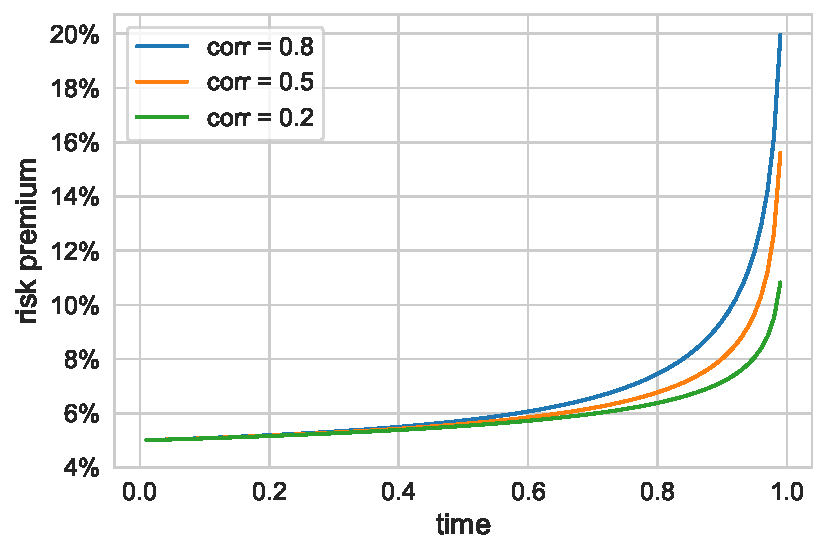
\includegraphics[scale=0.8]{Figures/RiskPremia.pdf}
\end{center}
\end{figure}
